\chapter{Optimization Results}
\label{sec:optimization_results}
This chapter focuses on showing and analyzing the most interesting MAV designs
outputted by the optimization tool. A short digression on platonic solid is first
needed to properly analyse the results. The optimal designs with an even number
of propellers are then described. Afterwards, the designs with an odd number of
propellers are shown. A comparison of the different optimal drone design is then
proposed. Finally, a few results of optimizations performed with the number of
propeller as an argument are presented.

\section{Platonic Solids}
\label{sec:platonic_solids}
Platonic solids are five regular and convex polyhedrons named after the
ancient Greek philosopher Plato to honor his memory \citep{noauthor_platonic_2018}.
The five platonic solids are:
\begin{itemize}
\item The tetrahedron composed of four faces and four vertices (see \Cref{fig:tetrahedron}).
\item The octahedron composed of eight faces and six vertices (see \Cref{fig:octahedron}).
\item The cube composed of six faces and eight vertices (see \Cref{fig:cube}).
\item The icosahedron composed of twenty faces and twelve vertices.
\item The dodecahedron composed of twelve faces and twenty vertices.
\end{itemize}
There is a angle that can be found at least in the
first three platonic solids. This angle is found between the horizontal plane and
the vertices of the polyhedron (see \Cref{fig:platonic_solid}). To ensure simplicity,
in the rest of this work this angle will be referred to as the platonic solids angle
and $\beta_{PS}$).

\begin{figure}[!h]
  \begin{subfigure}[b]{0.22\textwidth}
    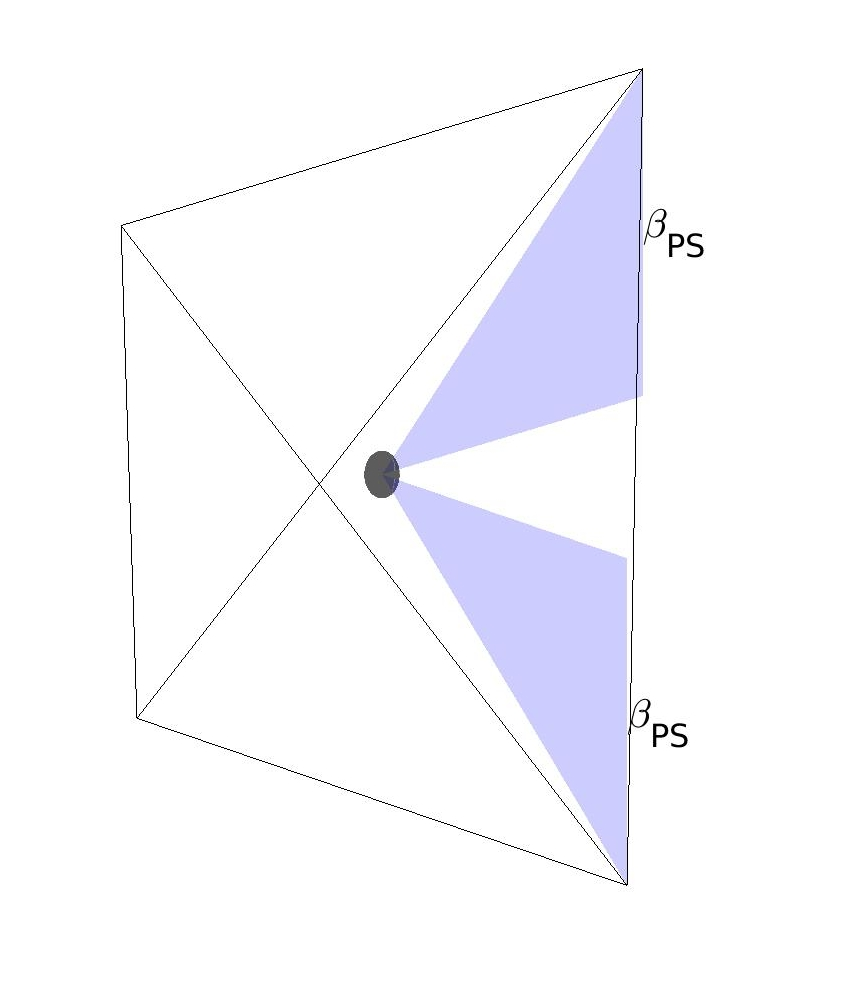
\includegraphics[width=\linewidth]{images/tetrahedron.jpg}
    \caption{Tetrahedron.} \label{fig:tetrahedron}
  \end{subfigure}
  \hspace*{\fill} % separation between the subfigures
  \begin{subfigure}[b]{0.27\textwidth}
    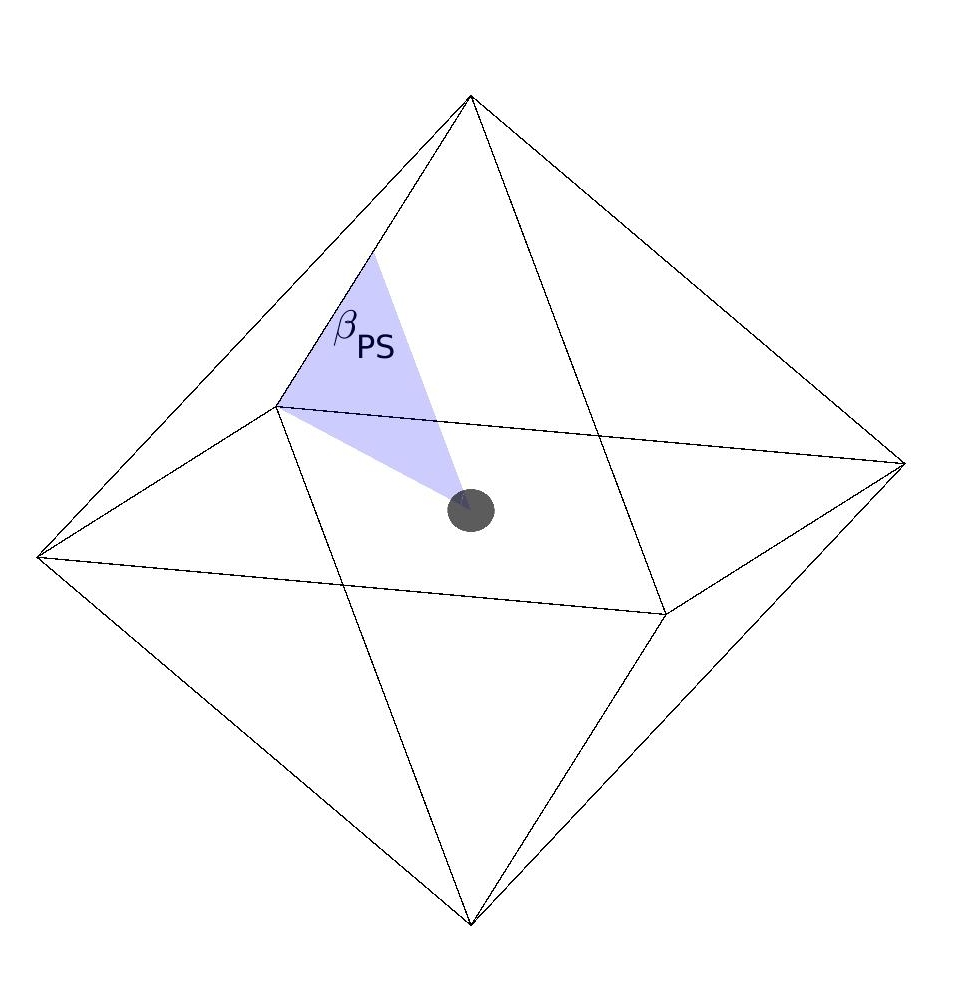
\includegraphics[width=\linewidth]{images/octahedron.jpg}
    \caption{Octahedron.} \label{fig:octahedron}
  \end{subfigure}
  \hspace*{\fill} % separation between the subfigures
  \begin{subfigure}[b]{0.26\textwidth}
    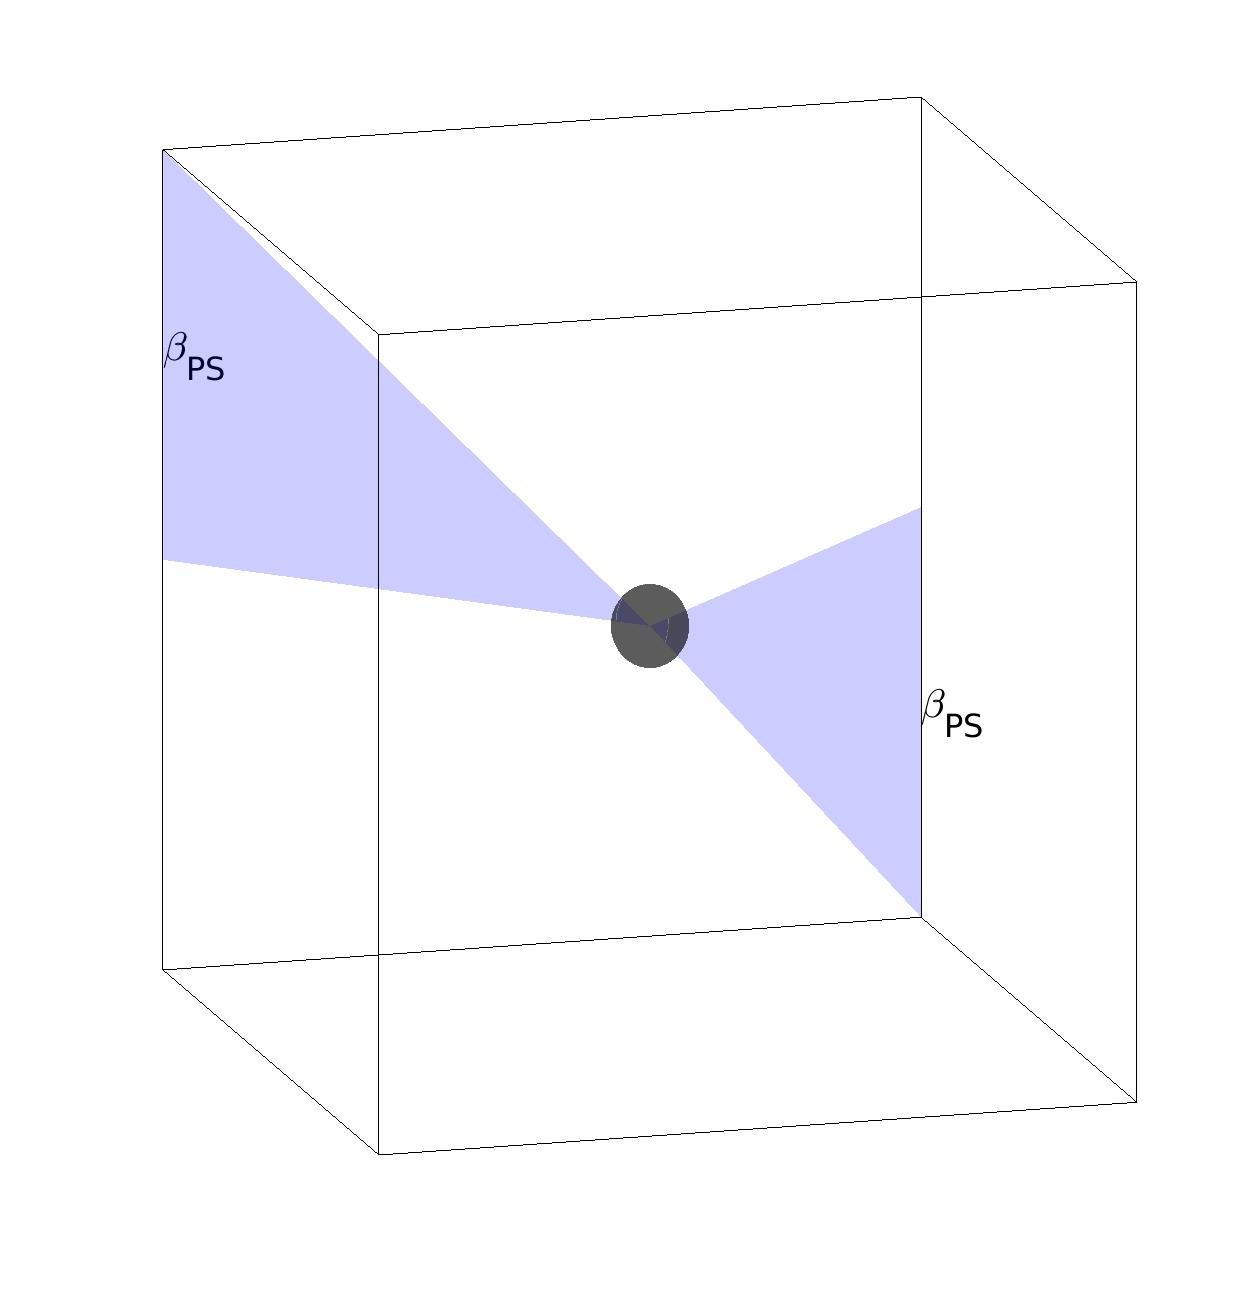
\includegraphics[width=\linewidth]{images/cube.jpg}
    \caption{Cube.} \label{fig:cube}
  \end{subfigure}
  \caption{The first three platonic solids $\big(\cos(\beta_{PS}) = \sqrt{\frac{2}{3}}
  =>  \beta_{PS} \simeq 35.26^{\circ}\big)\, .$}
  \label{fig:platonic_solid}
\end{figure}



\section{Even Designs}
\label{sec:even_designs}

\subsection{Quad-copter}
\label{sec:quad_copter}

\begin{figure}[!h]
  \resizebox{\textwidth}{!}{\begin{subfigure}[b]{0.55\textwidth}
    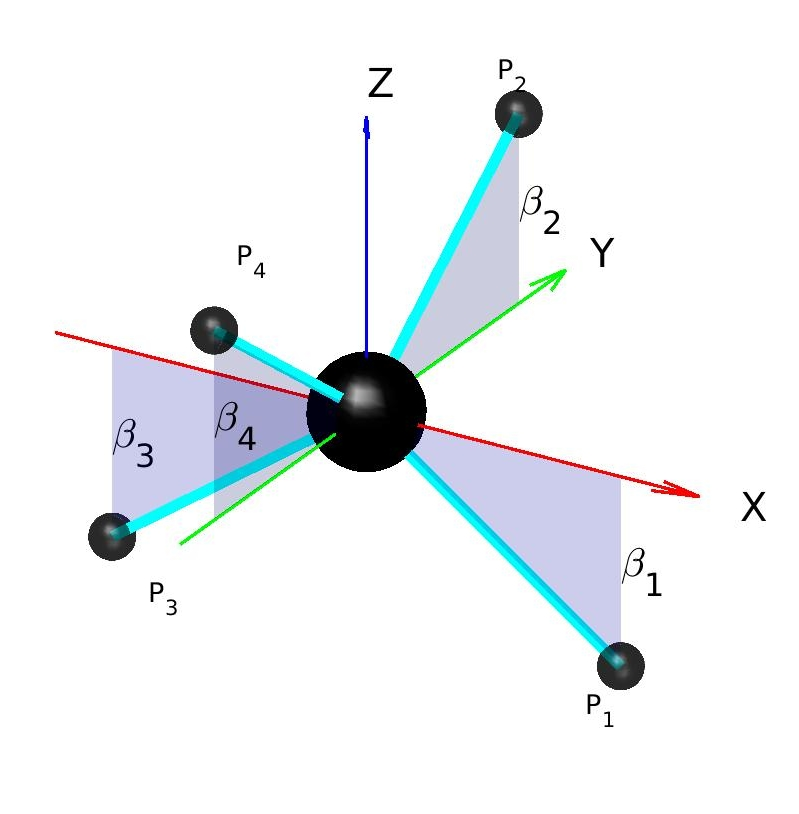
\includegraphics[width=\linewidth]{images/Quadcopter.jpg}
    \caption{$\beta\ =\ [35.26^{\circ}, -35.26^{\circ}, 35.26^{\circ},
    -35.26^{\circ}]$.} \label{fig:Quadcopter_resulta}
  \end{subfigure}
  \hspace*{\fill} % separation between the subfigures
  \begin{subfigure}[b]{0.5\textwidth}
    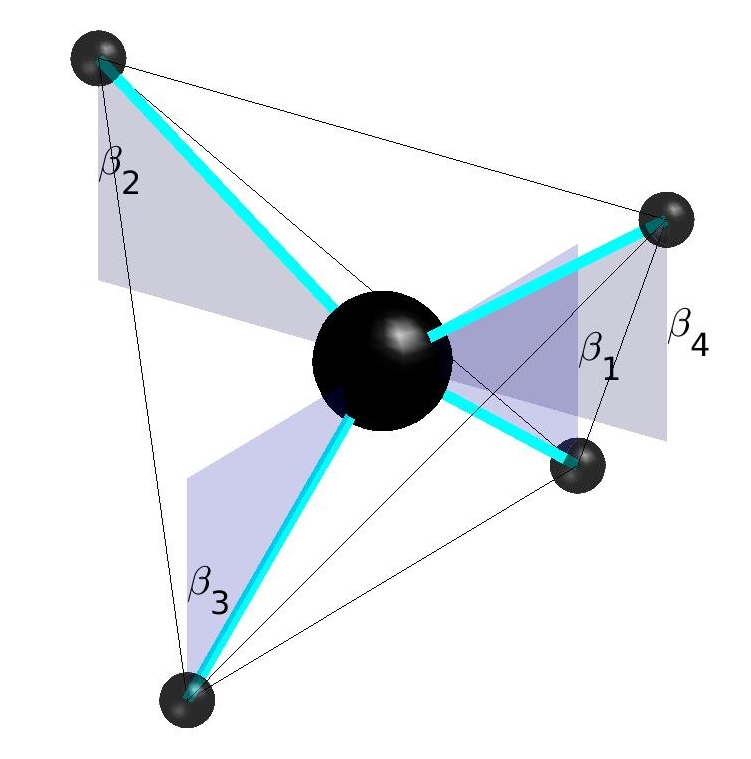
\includegraphics[width=\linewidth]{images/Quad_tetrahedron.jpg}
    \caption{Within a tetrahedron.} \label{fig:Quadcopter_resultb}
  \end{subfigure}}
  \caption{Schematic of the design obtained for the Quadcopter.}
  \label{fig:Quadcopter_result}
\end{figure}

\begin{figure}[!h]
  \resizebox{\textwidth}{!}{\begin{subfigure}[b]{0.55\textwidth}
    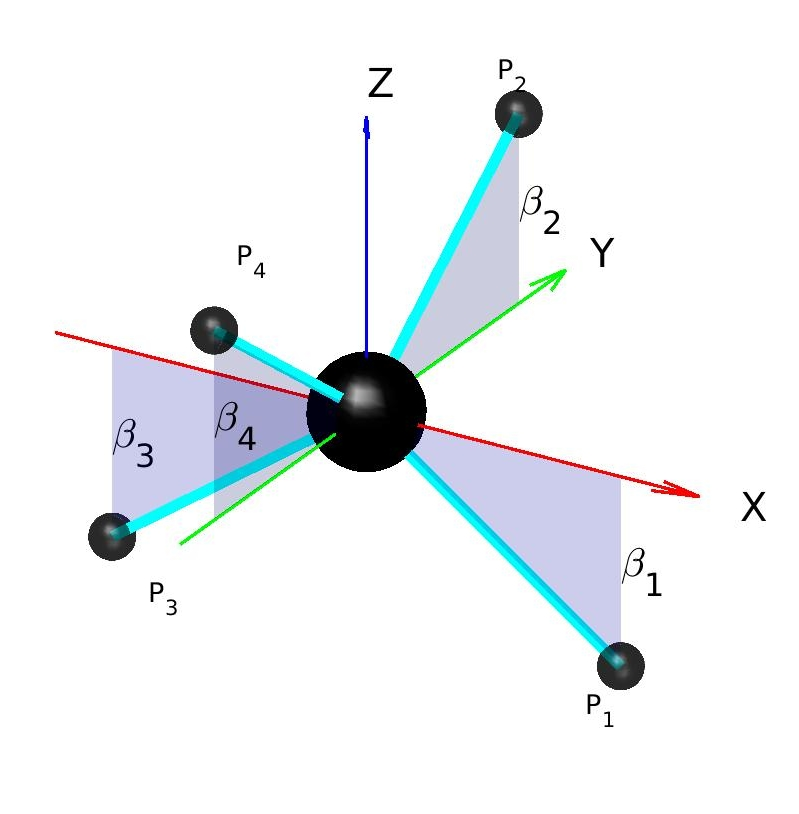
\includegraphics[width=\linewidth]{images/Quadcopter.jpg}
    \caption{$\beta\ =\ [35.26^{\circ}, -35.26^{\circ}, 35.26^{\circ},
    -35.26^{\circ}]$.} \label{fig:Quadcopter_deisgn1}
  \end{subfigure}
  \hspace*{\fill} % separation between the subfigures
  \begin{subfigure}[b]{0.6\textwidth}
    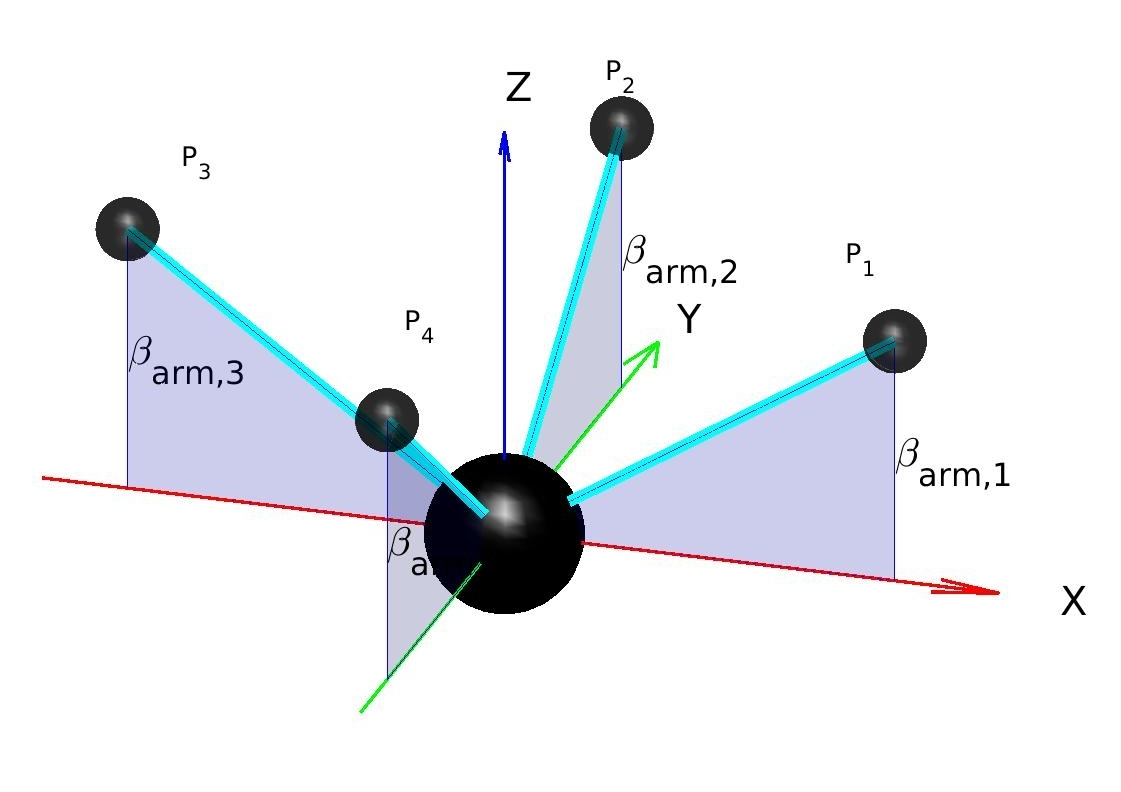
\includegraphics[width=\linewidth]{images/Quadcopter2.jpg}
    \caption{$\beta\ =\ [-32.42^{\circ}, -35.49^{\circ}, -35.44^{\circ},
    -35.49^{\circ}]$.} \label{fig:Quadcopter_deisgn2}
  \end{subfigure}}
  \caption{Schematic of the design obtained for the Quadcopter.}
  \label{fig:Quadcopter_equivalent}
\end{figure}

\subsection{Hexa-copter}
\label{sec:hexa_copter}

\subsection{Octa-copter}
\label{sec:octa_copter}

\section{Odd Designs}
\label{sec:odd_designs}

\subsection{Tri-copter}
\label{sec:tri_copter}
Show tricopter.

\subsection{Penta-copter}
\label{sec:penta_copter}

\subsection{Hepta-copter}
\label{sec:hepta_copter}

\section{Comparison of Different Designs}
\label{sec:comparison}
%\chapter{Einleitung}
%\label{sec:einleitung}
\section{Results when n is an Optimization Parameter}
\label{sec:result_n}

$F_{min} = 34.74, F_{max} = 42.55 , M_{min} = 17.42,  M_{max} = 21.34,  H_{eff,min} = 81.65\%,  H_{eff,max} = 100\%$\\
$F_{min} = 26.6, F_{max} = 52.11 , M_{min} = 15.1,  M_{max} = 26.13,  H_{eff,min} = 75\%,  H_{eff,max} = 100\%$\\
Design 1: $F_{min} = 23.18, F_{max} = 28.56 , M_{min} = 11.61,  M_{max} = 14.3,  H_{eff,min} = 81.11\%,  H_{eff,max} = 95.2\%$\\
Design 2: $F_{min} = 23.22, F_{max} = 28.37 , M_{min} = 11.65,  M_{max} = 14.23,  H_{eff,min} = 81.65\%, H_{eff,max} = 94.73\%$\\
$F_{min} = 44.7, F_{max} = 58.8 , M_{min} = 22.4,  M_{max} = 29.5,  H_{eff,min} = 81.78\%,  H_{eff,max} = 96.65\%$\\
$F_{min} = 46.46, F_{max} = 56.73 , M_{min} = 23.3,  M_{max} = 28.45,  H_{eff,min} = 81.64\%, H_{eff,max} = 94.77\%$\\

\begin{table}[h]
\begin{center}
 \caption{Comparison between the different number of propellers.}\vspace{1ex}
 \label{tab:tabnefz}
 \begin{tabular}{l|ccccccccc}
 \hline
 MAV Design & $F_{min} [N]$ & $F_{max} [N]$ & $F_{mean} [N]$ & $M_{min} [Nm]$ & $M_{max} [Nm]$ & $M_{mean} [Nm]$ & $H_{eff,mean} [\%]$ \\ \hline \hline
 Tri-copter  & 17.17 & 21.21 & 17.95 & 8.61 & 10.64 & 9 & 85.46\\
 Quad-copter & 23.22 & 28.37 & 26.87 & 11.65 & 14.23 & 13.47& 87.1 \\
 Penta-copter  & 28.95 & 35.46 & 29.4 & 14.52 & 17.78 & 14.74 & 85.35\\
 Hexa-copter  & 34.74 & 42.55 & 39.52 & 17.42 & 21.34 & 19.82 & 88.9\\
 Hepta-copter  & 39.96 & 49.44 & 47.2 & 20.04 & 24.8 & 23.66 & 91.1\\
 Octa-copter  & 44.7 & 58.8 & 53.95 & 22.4 & 29.48 & 27.06 & 91.42\\
 \hline
 \end{tabular}
\end{center}
\end{table}
